\documentclass[]{book}
\usepackage{lmodern}
\usepackage{amssymb,amsmath}
\usepackage{ifxetex,ifluatex}
\usepackage{fixltx2e} % provides \textsubscript
\ifnum 0\ifxetex 1\fi\ifluatex 1\fi=0 % if pdftex
  \usepackage[T1]{fontenc}
  \usepackage[utf8]{inputenc}
\else % if luatex or xelatex
  \ifxetex
    \usepackage{mathspec}
  \else
    \usepackage{fontspec}
  \fi
  \defaultfontfeatures{Ligatures=TeX,Scale=MatchLowercase}
\fi
% use upquote if available, for straight quotes in verbatim environments
\IfFileExists{upquote.sty}{\usepackage{upquote}}{}
% use microtype if available
\IfFileExists{microtype.sty}{%
\usepackage{microtype}
\UseMicrotypeSet[protrusion]{basicmath} % disable protrusion for tt fonts
}{}
\usepackage[margin=1in]{geometry}
\usepackage{hyperref}
\hypersetup{unicode=true,
            pdftitle={Collaborative Data Science Practices},
            pdfauthor={Will Beasley},
            pdfborder={0 0 0},
            breaklinks=true}
\urlstyle{same}  % don't use monospace font for urls
\usepackage{natbib}
\bibliographystyle{apalike}
\usepackage{color}
\usepackage{fancyvrb}
\newcommand{\VerbBar}{|}
\newcommand{\VERB}{\Verb[commandchars=\\\{\}]}
\DefineVerbatimEnvironment{Highlighting}{Verbatim}{commandchars=\\\{\}}
% Add ',fontsize=\small' for more characters per line
\usepackage{framed}
\definecolor{shadecolor}{RGB}{248,248,248}
\newenvironment{Shaded}{\begin{snugshade}}{\end{snugshade}}
\newcommand{\AlertTok}[1]{\textcolor[rgb]{0.94,0.16,0.16}{#1}}
\newcommand{\AnnotationTok}[1]{\textcolor[rgb]{0.56,0.35,0.01}{\textbf{\textit{#1}}}}
\newcommand{\AttributeTok}[1]{\textcolor[rgb]{0.77,0.63,0.00}{#1}}
\newcommand{\BaseNTok}[1]{\textcolor[rgb]{0.00,0.00,0.81}{#1}}
\newcommand{\BuiltInTok}[1]{#1}
\newcommand{\CharTok}[1]{\textcolor[rgb]{0.31,0.60,0.02}{#1}}
\newcommand{\CommentTok}[1]{\textcolor[rgb]{0.56,0.35,0.01}{\textit{#1}}}
\newcommand{\CommentVarTok}[1]{\textcolor[rgb]{0.56,0.35,0.01}{\textbf{\textit{#1}}}}
\newcommand{\ConstantTok}[1]{\textcolor[rgb]{0.00,0.00,0.00}{#1}}
\newcommand{\ControlFlowTok}[1]{\textcolor[rgb]{0.13,0.29,0.53}{\textbf{#1}}}
\newcommand{\DataTypeTok}[1]{\textcolor[rgb]{0.13,0.29,0.53}{#1}}
\newcommand{\DecValTok}[1]{\textcolor[rgb]{0.00,0.00,0.81}{#1}}
\newcommand{\DocumentationTok}[1]{\textcolor[rgb]{0.56,0.35,0.01}{\textbf{\textit{#1}}}}
\newcommand{\ErrorTok}[1]{\textcolor[rgb]{0.64,0.00,0.00}{\textbf{#1}}}
\newcommand{\ExtensionTok}[1]{#1}
\newcommand{\FloatTok}[1]{\textcolor[rgb]{0.00,0.00,0.81}{#1}}
\newcommand{\FunctionTok}[1]{\textcolor[rgb]{0.00,0.00,0.00}{#1}}
\newcommand{\ImportTok}[1]{#1}
\newcommand{\InformationTok}[1]{\textcolor[rgb]{0.56,0.35,0.01}{\textbf{\textit{#1}}}}
\newcommand{\KeywordTok}[1]{\textcolor[rgb]{0.13,0.29,0.53}{\textbf{#1}}}
\newcommand{\NormalTok}[1]{#1}
\newcommand{\OperatorTok}[1]{\textcolor[rgb]{0.81,0.36,0.00}{\textbf{#1}}}
\newcommand{\OtherTok}[1]{\textcolor[rgb]{0.56,0.35,0.01}{#1}}
\newcommand{\PreprocessorTok}[1]{\textcolor[rgb]{0.56,0.35,0.01}{\textit{#1}}}
\newcommand{\RegionMarkerTok}[1]{#1}
\newcommand{\SpecialCharTok}[1]{\textcolor[rgb]{0.00,0.00,0.00}{#1}}
\newcommand{\SpecialStringTok}[1]{\textcolor[rgb]{0.31,0.60,0.02}{#1}}
\newcommand{\StringTok}[1]{\textcolor[rgb]{0.31,0.60,0.02}{#1}}
\newcommand{\VariableTok}[1]{\textcolor[rgb]{0.00,0.00,0.00}{#1}}
\newcommand{\VerbatimStringTok}[1]{\textcolor[rgb]{0.31,0.60,0.02}{#1}}
\newcommand{\WarningTok}[1]{\textcolor[rgb]{0.56,0.35,0.01}{\textbf{\textit{#1}}}}
\usepackage{longtable,booktabs}
\usepackage{graphicx,grffile}
\makeatletter
\def\maxwidth{\ifdim\Gin@nat@width>\linewidth\linewidth\else\Gin@nat@width\fi}
\def\maxheight{\ifdim\Gin@nat@height>\textheight\textheight\else\Gin@nat@height\fi}
\makeatother
% Scale images if necessary, so that they will not overflow the page
% margins by default, and it is still possible to overwrite the defaults
% using explicit options in \includegraphics[width, height, ...]{}
\setkeys{Gin}{width=\maxwidth,height=\maxheight,keepaspectratio}
\IfFileExists{parskip.sty}{%
\usepackage{parskip}
}{% else
\setlength{\parindent}{0pt}
\setlength{\parskip}{6pt plus 2pt minus 1pt}
}
\setlength{\emergencystretch}{3em}  % prevent overfull lines
\providecommand{\tightlist}{%
  \setlength{\itemsep}{0pt}\setlength{\parskip}{0pt}}
\setcounter{secnumdepth}{5}
% Redefines (sub)paragraphs to behave more like sections
\ifx\paragraph\undefined\else
\let\oldparagraph\paragraph
\renewcommand{\paragraph}[1]{\oldparagraph{#1}\mbox{}}
\fi
\ifx\subparagraph\undefined\else
\let\oldsubparagraph\subparagraph
\renewcommand{\subparagraph}[1]{\oldsubparagraph{#1}\mbox{}}
\fi

%%% Use protect on footnotes to avoid problems with footnotes in titles
\let\rmarkdownfootnote\footnote%
\def\footnote{\protect\rmarkdownfootnote}

%%% Change title format to be more compact
\usepackage{titling}

% Create subtitle command for use in maketitle
\newcommand{\subtitle}[1]{
  \posttitle{
    \begin{center}\large#1\end{center}
    }
}

\setlength{\droptitle}{-2em}

  \title{Collaborative Data Science Practices}
    \pretitle{\vspace{\droptitle}\centering\huge}
  \posttitle{\par}
    \author{Will Beasley}
    \preauthor{\centering\large\emph}
  \postauthor{\par}
      \predate{\centering\large\emph}
  \postdate{\par}
    \date{2019-02-11}

\usepackage{booktabs}

\begin{document}
\maketitle

{
\setcounter{tocdepth}{1}
\tableofcontents
}
\hypertarget{prerequisites}{%
\chapter{Prerequisites}\label{prerequisites}}

This is a \emph{sample} book written in \textbf{Markdown}. You can use anything that Pandoc's Markdown supports, e.g., a math equation \(a^2 + b^2 = c^2\).

The \textbf{bookdown} package can be installed from CRAN or Github:

\begin{Shaded}
\begin{Highlighting}[]
\KeywordTok{install.packages}\NormalTok{(}\StringTok{"bookdown"}\NormalTok{)}
\CommentTok{# or the development version}
\CommentTok{# devtools::install_github("rstudio/bookdown")}
\end{Highlighting}
\end{Shaded}

Remember each Rmd file contains one and only one chapter, and a chapter is defined by the first-level heading \texttt{\#}.

To compile this example to PDF, you need XeLaTeX. You are recommended to install TinyTeX (which includes XeLaTeX): \url{https://yihui.name/tinytex/}.

\hypertarget{architecture}{%
\chapter{Architecture Principles}\label{architecture}}

\hypertarget{encapsulation}{%
\section{Encapsulation}\label{encapsulation}}

\hypertarget{leverage-team-members-strenghts-avoid-weaknesses}{%
\section{Leverage team member's strenghts \& avoid weaknesses}\label{leverage-team-members-strenghts-avoid-weaknesses}}

\begin{enumerate}
\def\labelenumi{\arabic{enumi}.}
\tightlist
\item
  Focused code files
\item
  Metadata for content experts
\end{enumerate}

\hypertarget{scales}{%
\section{Scales}\label{scales}}

\begin{enumerate}
\def\labelenumi{\arabic{enumi}.}
\tightlist
\item
  Single source \& single analysis
\item
  Multiple sources \& multiple analyses
\end{enumerate}

\hypertarget{consistency}{%
\section{Consistency}\label{consistency}}

\begin{enumerate}
\def\labelenumi{\arabic{enumi}.}
\tightlist
\item
  Across Files \{\#consistency-files\}
\item
  Across Languages
\item
  Across Projects
\end{enumerate}

\hypertarget{file-prototype}{%
\chapter{Prototypical File}\label{file-prototype}}

As stated before, in \protect\hyperlink{consistency-files}{Consistency Files}, using a consistent file structure can (a) improve the quality of the code because the structure has been proven over time to facilitate good practices and (b) allow your intentions to be more clear to teammates because they are familiar with the order and intentions of the chunks.

We use the term ``chunk'' for a section of code because it corresponds with knitr terminology \citep{xie2015}, and in many cases, the chunk of our R file connects to a knitr Rmd file.

\hypertarget{clear-memory}{%
\section{Clear Memory}\label{clear-memory}}

\hypertarget{load-sources}{%
\section{Load Sources}\label{load-sources}}

\hypertarget{load-packages}{%
\section{Load Packages}\label{load-packages}}

\hypertarget{declare-globals}{%
\section{Declare Globals}\label{declare-globals}}

\hypertarget{load-data}{%
\section{Load Data}\label{load-data}}

\hypertarget{tweak-data}{%
\section{Tweak Data}\label{tweak-data}}

\hypertarget{unique-content}{%
\section{(Unique Content)}\label{unique-content}}

\hypertarget{verify-values}{%
\section{Verify Values}\label{verify-values}}

\hypertarget{specify-output-columns}{%
\section{Specify Output Columns}\label{specify-output-columns}}

\hypertarget{save-to-disk-or-database}{%
\section{Save to Disk or Database}\label{save-to-disk-or-database}}

\hypertarget{repo-prototype}{%
\chapter{Prototypical Repository}\label{repo-prototype}}

\url{https://github.com/wibeasley/RAnalysisSkeleton}

\hypertarget{analysis}{%
\section{Analysis}\label{analysis}}

\hypertarget{data-public}{%
\section{Data Public}\label{data-public}}

\begin{enumerate}
\def\labelenumi{\arabic{enumi}.}
\tightlist
\item
  Raw
\item
  Derived
\item
  Metadata
\item
  Database
\item
  Original
\end{enumerate}

\hypertarget{data-unshared}{%
\section{Data Unshared}\label{data-unshared}}

\hypertarget{documentation}{%
\section{Documentation}\label{documentation}}

\hypertarget{manipulation}{%
\section{Manipulation}\label{manipulation}}

\hypertarget{stitched-output}{%
\section{Stitched Output}\label{stitched-output}}

\hypertarget{utility}{%
\section{Utility}\label{utility}}

\hypertarget{data-at-rest}{%
\chapter{Data at Rest}\label{data-at-rest}}

\hypertarget{data-states}{%
\section{Data States}\label{data-states}}

\begin{enumerate}
\def\labelenumi{\arabic{enumi}.}
\tightlist
\item
  Raw
\item
  Derived

  \begin{enumerate}
  \def\labelenumii{\arabic{enumii}.}
  \tightlist
  \item
    Project-wide File on Repo
  \item
    Project-wide File on Protected File Server
  \item
    User-specific File on Protected File Server
  \item
    Project-wide Database
  \end{enumerate}
\item
  Original
\end{enumerate}

\hypertarget{data-containers}{%
\section{Data Containers}\label{data-containers}}

\begin{enumerate}
\def\labelenumi{\arabic{enumi}.}
\tightlist
\item
  csv
\item
  rds
\item
  SQLite
\item
  Central Enterprise database
\item
  Central REDCap database
\item
  Containers to avoid for raw/input

  \begin{enumerate}
  \def\labelenumii{\arabic{enumii}.}
  \tightlist
  \item
    Proprietary like xlsx, sas7bdat
  \end{enumerate}
\end{enumerate}

\hypertarget{patterns}{%
\chapter{Patterns}\label{patterns}}

\hypertarget{ellis}{%
\section{Ellis}\label{ellis}}

\hypertarget{purpose}{%
\subsection{Purpose}\label{purpose}}

To incorporate outside data source into your system safely.

\hypertarget{philosophy}{%
\subsection{Philosophy}\label{philosophy}}

\begin{itemize}
\tightlist
\item
  Without data immigration, all warehouses are useless. Embrace the power of fresh information in a way that is:

  \begin{itemize}
  \tightlist
  \item
    repeatable when the datasource is updated (and you have to refresh your warehouse)
  \item
    similar to other Ellis lanes (that are designed for other data sources) so you don't have to learn/remember an entirely new pattern. (Like Rubiks cube instructions.)
  \end{itemize}
\end{itemize}

\hypertarget{guidelines}{%
\subsection{Guidelines}\label{guidelines}}

\begin{itemize}
\tightlist
\item
  Take small bites.

  \begin{itemize}
  \tightlist
  \item
    Like all software development, don't tackle all the complexity the first time. Start by processing only the important columns before incorporating move.
  \item
    Use only the variables you need in the short-term, especially for new projects. As everyone knows, the variables from the upstream source can change. Don't spend effort writing code for variables you won't need for a few months/years; they'll likely change before you need them.
  \item
    After a row passes through the \texttt{verify-values} chunk, you're accountable for any failures it causes in your warehouse. All analysts know that external data is messy, so don't be surprised. Sometimes I'll spend an hour writing an Ellis for 6 columns.
  \end{itemize}
\item
  Narrowly define each Ellis lane. One code file should strive to (a) consume only one CSV and (b) produce only one table. Exceptions include:

  \begin{enumerate}
  \def\labelenumi{\arabic{enumi}.}
  \tightlist
  \item
    if multiple input files are related, and really belong together (\emph{e.g.}, one CSV per month, or one CSV per clinic). This scenario is pretty common.
  \item
    if the CSV should legitimately produce two different tables after munging. This happens infrequently, such as one warehouse table needs to be wide, and another long.
  \end{enumerate}
\end{itemize}

\hypertarget{examples}{%
\subsection{Examples}\label{examples}}

\begin{itemize}
\tightlist
\item
  \url{https://github.com/wibeasley/RAnalysisSkeleton/blob/master/manipulation/te-ellis.R}
\item
  \url{https://github.com/wibeasley/RAnalysisSkeleton/blob/master/manipulation/}
\item
  \url{https://github.com/OuhscBbmc/usnavy-billets/blob/master/manipulation/survey-ellis.R}
\end{itemize}

\hypertarget{elements}{%
\subsection{Elements}\label{elements}}

\begin{enumerate}
\def\labelenumi{\arabic{enumi}.}
\item
  \textbf{Clear memory} In scripting languages like R (unlike compiled languages like Java), it's easy for old variables to hang around. Explicitly clear them before you run the file again.

\begin{Shaded}
\begin{Highlighting}[]
\KeywordTok{rm}\NormalTok{(}\DataTypeTok{list=}\KeywordTok{ls}\NormalTok{(}\DataTypeTok{all=}\OtherTok{TRUE}\NormalTok{)) }\CommentTok{#Clear the memory of variables from previous run. This is not called by knitr, because it's above the first chunk.}
\end{Highlighting}
\end{Shaded}
\item
  \textbf{Load Sources} In R, a \texttt{source()}d file is run to execute its code. We prefer that a sourced file only load variables (like function definitions), instead of do real operations like read a dataset or perform a calculation. There are many times that you want a function to be available to multiple files in a repo; there are two approaches we like. The first is collecting those common functions into a single file (and then sourcing it in the callers). The second is to make the repo a legitimate R package.

  The first approach is better suited for quick \& easy development. The second allows you to add documention and unit tests.

\begin{Shaded}
\begin{Highlighting}[]
\CommentTok{# ---- load-sources ------------------------------------------------------------}
\KeywordTok{source}\NormalTok{(}\StringTok{"./manipulation/osdh/ellis/common-ellis.R"}\NormalTok{)}
\end{Highlighting}
\end{Shaded}
\item
  \textbf{Load Packages} This is another precaution necessary in a scripting language. Determine if the necessary packages are available on the machine. Avoiding attaching packages (with the \texttt{library()} function) when possible. Their functions don't need to be qualified (\emph{e.g.}, \texttt{dplyr::intersect()}) and could cause naming conflicts. Even if you can guarantee they don't conflict with packages now, packages could add new functions in the future that do conflict.

\begin{Shaded}
\begin{Highlighting}[]
\CommentTok{# ---- load-packages -----------------------------------------------------------}
\CommentTok{# Attach these package(s) so their functions don't need to be qualified: http://r-pkgs.had.co.nz/namespace.html#search-path}
\KeywordTok{library}\NormalTok{(magrittr            , }\DataTypeTok{quietly=}\OtherTok{TRUE}\NormalTok{)}
\KeywordTok{library}\NormalTok{(DBI                 , }\DataTypeTok{quietly=}\OtherTok{TRUE}\NormalTok{)}

\CommentTok{# Verify these packages are available on the machine, but their functions need to be qualified: http://r-pkgs.had.co.nz/namespace.html#search-path}
\KeywordTok{requireNamespace}\NormalTok{(}\StringTok{"readr"}\NormalTok{        )}
\KeywordTok{requireNamespace}\NormalTok{(}\StringTok{"tidyr"}\NormalTok{        )}
\KeywordTok{requireNamespace}\NormalTok{(}\StringTok{"dplyr"}\NormalTok{        ) }\CommentTok{# Avoid attaching dplyr, b/c its function names conflict with a lot of packages (esp base, stats, and plyr).}
\KeywordTok{requireNamespace}\NormalTok{(}\StringTok{"testit"}\NormalTok{)}
\KeywordTok{requireNamespace}\NormalTok{(}\StringTok{"checkmate"}\NormalTok{)}
\KeywordTok{requireNamespace}\NormalTok{(}\StringTok{"OuhscMunge"}\NormalTok{) }\CommentTok{#devtools::install_github(repo="OuhscBbmc/OuhscMunge")}
\end{Highlighting}
\end{Shaded}
\item
  \textbf{Declare Global Variables and Functions}. This includes defining the expected column names and types of the data sources; use \texttt{readr::cols\_only()} (as opposed to \texttt{readr::cols()}) to ignore any new columns that may be been added since the dataset's last refresh.

\begin{Shaded}
\begin{Highlighting}[]
\CommentTok{# ---- declare-globals ---------------------------------------------------------}
\end{Highlighting}
\end{Shaded}
\item
  \textbf{Load Data Source(s)} Read all data (\emph{e.g.}, database table, networked CSV, local lookup table). After this chunk, no new data should be introduced. This is for the sake of reducing human cognition load. Everything below this chunk is derived from these first four chunks.

\begin{Shaded}
\begin{Highlighting}[]
\CommentTok{# ---- load-data ---------------------------------------------------------------}
\end{Highlighting}
\end{Shaded}
\item
  \textbf{Tweak Data}

\begin{Shaded}
\begin{Highlighting}[]
\CommentTok{# ---- tweak-data --------------------------------------------------------------}
\end{Highlighting}
\end{Shaded}
\item
  \textbf{Body of the Ellis}
\item
  \textbf{Verify}

\begin{Shaded}
\begin{Highlighting}[]
\CommentTok{# ---- verify-values -----------------------------------------------------------}
\NormalTok{county_month_combo   <-}\StringTok{ }\KeywordTok{paste}\NormalTok{(ds}\OperatorTok{$}\NormalTok{county_id, ds}\OperatorTok{$}\NormalTok{month)}
\NormalTok{checkmate}\OperatorTok{::}\KeywordTok{assert_character}\NormalTok{(county_month_combo, }\DataTypeTok{pattern  =}\StringTok{"^}\CharTok{\textbackslash{}\textbackslash{}}\StringTok{d\{1,2\} }\CharTok{\textbackslash{}\textbackslash{}}\StringTok{d\{4\}-}\CharTok{\textbackslash{}\textbackslash{}}\StringTok{d\{2\}-}\CharTok{\textbackslash{}\textbackslash{}}\StringTok{d\{2\}$"}\NormalTok{, }\DataTypeTok{any.missing=}\NormalTok{F, }\DataTypeTok{unique=}\NormalTok{T)}
\end{Highlighting}
\end{Shaded}
\item
  \textbf{Specify Columns} Define the exact columns and order to upload to the database. Once you import a column into a warehouse that multiple people are using, it's tough to remove it.

\begin{Shaded}
\begin{Highlighting}[]
\CommentTok{# ---- specify-columns-to-upload -----------------------------------------------}
\end{Highlighting}
\end{Shaded}
\item
  \textbf{Welcome} into your warehouse. Until this chunk, nothing should be persisted.

\begin{Shaded}
\begin{Highlighting}[]
\CommentTok{# ---- upload-to-db ------------------------------------------------------------}
\CommentTok{# ---- save-to-disk ------------------------------------------------------------}
\end{Highlighting}
\end{Shaded}
\end{enumerate}

\hypertarget{arch}{%
\section{Arch}\label{arch}}

\hypertarget{ferry}{%
\section{Ferry}\label{ferry}}

\hypertarget{scribe}{%
\section{Scribe}\label{scribe}}

\hypertarget{analysis-1}{%
\section{Analysis}\label{analysis-1}}

\hypertarget{presentation--static}{%
\section{Presentation -Static}\label{presentation--static}}

\hypertarget{presentation--interactive}{%
\section{Presentation -Interactive}\label{presentation--interactive}}

\hypertarget{metadata}{%
\section{Metadata}\label{metadata}}

\hypertarget{security}{%
\chapter{Security \& Private Data}\label{security}}

\hypertarget{file-level-permissions}{%
\section{File-level permissions}\label{file-level-permissions}}

\hypertarget{database-permissions}{%
\section{Database permissions}\label{database-permissions}}

\hypertarget{public-private-repositories}{%
\section{Public \& Private Repositories}\label{public-private-repositories}}

\hypertarget{scrubbing-github-history}{%
\subsection{Scrubbing GitHub history}\label{scrubbing-github-history}}

Occassionaly files may be committed to your git repository that need to be removed completely. Not just from the current collections of files (\emph{i.e.}, the branch's \href{https://git-scm.com/docs/gitglossary\#gitglossary-aiddefHEADaHEAD}{head}), but from the entire history of the repo.

Scrubbing is require typically when (a) a sensitive file has been accidentally commited and pushed to GitHub, or (b) a huge file has bloated your repository and disrupted productivity.

The two suitable scrubbing approaches both require the command line. The first is the \texttt{git-filter-branch} command within git, and the second is the \href{https://rtyley.github.io/bfg-repo-cleaner/}{BFG repo-cleaner}. We use the second approach, which is {[}recommended by GitHub{]}; it requires 15 minutes to install and configure from scratch, but then is much easier to develop against, and executes much faster.

The \href{https://www.gnu.org/software/bash/}{bash}-centric steps below remove any file\emph{s} from the repo history called `monster-data.csv' from the `bloated' repository.

\begin{enumerate}
\def\labelenumi{\arabic{enumi}.}
\item
  If the file contains passwords, change them immediately.
\item
  Delete `monster-data.csv' from your branch and push the commit to GitHub.
\item
  Ask your collaborators to push any outstanding commits to GitHub and delete their local copy of the repo. Once scrubbing is complete, they will re-clone it.
\item
  Download and install the most recent Java JRE from the Oracle site.
\item
  Download the most recent jar file from the BFG site to the home directory.
\item
  Clone a fresh copy of the repository in the user's home directory. The \texttt{-\/-mirror} argument avoids downloading every file, and downloads only the bookkeeping details required for scrubbing.

\begin{Shaded}
\begin{Highlighting}[]
\BuiltInTok{cd}\NormalTok{ ~}
\FunctionTok{git}\NormalTok{ clone --mirror https://github.com/your-org/bloated.git}
\end{Highlighting}
\end{Shaded}
\item
  Remove all files (in any directory) called `monster-data.csv'.

\begin{Shaded}
\begin{Highlighting}[]
\ExtensionTok{java}\NormalTok{ -jar bfg-*.jar --delete-files monster-data.csv bloated.git}
\end{Highlighting}
\end{Shaded}
\item
  \href{https://git-scm.com/docs/git-reflog}{Reflog} and \href{https://git-scm.com/docs/git-gc}{garbage collect} the repo.

\begin{Shaded}
\begin{Highlighting}[]
\BuiltInTok{cd}\NormalTok{ bloated.git}
\FunctionTok{git}\NormalTok{ reflog expire --expire=now --all }\KeywordTok{&&} \FunctionTok{git}\NormalTok{ gc --prune=now --aggressive}
\end{Highlighting}
\end{Shaded}
\item
  Push your local changes to the GitHub server.

\begin{Shaded}
\begin{Highlighting}[]
\FunctionTok{git}\NormalTok{ push}
\end{Highlighting}
\end{Shaded}
\item
  Delete the bfg jar from the home directory.

\begin{Shaded}
\begin{Highlighting}[]
\BuiltInTok{cd}\NormalTok{ ~}
\FunctionTok{rm}\NormalTok{ bfg-*.jar}
\end{Highlighting}
\end{Shaded}
\item
  Ask your collaborators to reclone the repo to their local machine. It is important they restart with a fresh copy, so the once-scrubbed file is not reintroduced into the repo's history.
\item
  If the file contains sensitive information, like passwords or PHI, ask GitHub to refresh the cache so the file's history isn't accessible through their website, even if the repo is private.
\end{enumerate}

\hypertarget{resources}{%
\paragraph{Resources}\label{resources}}

\begin{itemize}
\tightlist
\item
  \href{https://rtyley.github.io/bfg-repo-cleaner/}{BFG Repo-Cleaner site}
\item
  \href{https://github.com/IBM/BluePic/wiki/Using-BFG-Repo-Cleaner-tool-to-remove-sensitive-files-from-your-git-repo}{Additional BFG instructions}
\item
  \href{https://help.github.com/articles/github-sensitive-data-removal-policy/}{GitHub Sensitive Data Removal Policy}
\end{itemize}

\hypertarget{automation}{%
\chapter{Automation}\label{automation}}

\hypertarget{flow-file-in-r}{%
\section{Flow File in R}\label{flow-file-in-r}}

\hypertarget{makefile}{%
\section{Makefile}\label{makefile}}

\hypertarget{ssis}{%
\section{SSIS}\label{ssis}}

\hypertarget{cron-jobs-task-scheduler}{%
\section{cron Jobs \& Task Scheduler}\label{cron-jobs-task-scheduler}}

\hypertarget{sink-log-files}{%
\section{Sink Log Files}\label{sink-log-files}}

\hypertarget{scaling-up}{%
\chapter{Scaling Up}\label{scaling-up}}

\hypertarget{data-storage}{%
\section{Data Storage}\label{data-storage}}

\begin{enumerate}
\def\labelenumi{\arabic{enumi}.}
\tightlist
\item
  Local File vs Conventional Database vs Redshift
\item
  Usage Cases
\end{enumerate}

\hypertarget{data-processing}{%
\section{Data Processing}\label{data-processing}}

\begin{enumerate}
\def\labelenumi{\arabic{enumi}.}
\tightlist
\item
  R vs SQL
\item
  R vs Spark
\end{enumerate}

\hypertarget{collaboration}{%
\chapter{Parallel Collaboration}\label{collaboration}}

\hypertarget{social-contract}{%
\section{Social Contract}\label{social-contract}}

\begin{enumerate}
\def\labelenumi{\arabic{enumi}.}
\tightlist
\item
  Issues
\item
  Organized Commits \& Coherent Diffs
\item
  Branch \& Merge Strategy
\end{enumerate}

\hypertarget{code-reviews}{%
\section{Code Reviews}\label{code-reviews}}

\begin{enumerate}
\def\labelenumi{\arabic{enumi}.}
\tightlist
\item
  Daily Reviews of PRs
\item
  Periodic Reviews of Files
\end{enumerate}

\hypertarget{remote}{%
\section{Remote}\label{remote}}

\begin{enumerate}
\def\labelenumi{\arabic{enumi}.}
\tightlist
\item
  Headset \& sharing screens
\end{enumerate}

\hypertarget{document}{%
\chapter{Documentation}\label{document}}

\hypertarget{team-wide}{%
\section{Team-wide}\label{team-wide}}

\hypertarget{project-specific}{%
\section{Project-specific}\label{project-specific}}

\hypertarget{dataset-origin-structure}{%
\section{Dataset Origin \& Structure}\label{dataset-origin-structure}}

\hypertarget{issues-tasks}{%
\section{Issues \& Tasks}\label{issues-tasks}}

\hypertarget{flow-diagrams}{%
\section{Flow Diagrams}\label{flow-diagrams}}

\hypertarget{setting-up-new-machine}{%
\section{Setting up new machine}\label{setting-up-new-machine}}

(\href{https://github.com/OuhscBbmc/RedcapExamplesAndPatterns/blob/master/DocumentationGlobal/ResourcesInstallation.md}{example})

\hypertarget{style-guide}{%
\chapter{Style Guide}\label{style-guide}}

Using a consistent style across your projects can increase the overhead as your data science team discusses options, decides on a good choice, and develops in compliant code. But like in most themes in this document, the cost is worth the effort. Unforced code errors are reduced when code is consistent, because mistake-prone styles are more apparent.

For the most part, our team follows the \href{http://adv-r.had.co.nz/Style.html}{tidyverse style}. Here are some additional conventions we attempt to follow.

\hypertarget{ggplot2}{%
\section{ggplot2}\label{ggplot2}}

The expressiveness of \href{https://ggplot2.tidyverse.org/}{ggplot2} allows someone to quickly develop precise scientific graphics. One graph can be specified in many equivalent styles, which increases the opportunity for confusion. We formalized much of this style while writing a \href{https://github.com/OuhscBbmc/DeSheaToothakerIntroStats/blob/master/thumbnails/thumbnails.md}{textbook for introductory statistics}; the 200+ graphs and their code is publically available.

\hypertarget{order-of-commands}{%
\subsection{Order of commands}\label{order-of-commands}}

ggplot2 is essentially a collection of functions combined with the \texttt{+} operator. Publication graphs common require at least 20 functions, which means the functions can sometimes be redundant or step on each other toes. The family of functoins should follow a consistent order ideally starting with the more important structural functions and ending with the cosmetic functions. Our preference is:

\begin{enumerate}
\def\labelenumi{\arabic{enumi}.}
\tightlist
\item
  \texttt{ggplot2()} is the primary function to specify the default dataset and aesthetic mappings. Many arguments can be passed to \texttt{aes()}, and we prefer to follow an order consistent with the \texttt{scale\_*()} order below.
\item
  \texttt{geom\_*()} creates the \emph{geom}etric elements that reperesent the data. Unlike most categories in this list, the order matters. Geoms specified first are drawn first, and therefore can be obscured by subsequent geoms.
\item
  \texttt{scale\_*()} describes how a dimension of data (specified in \texttt{aes()}) is translated into a visual element. We specify the dimensions in descending order of (typical) importance: \texttt{x}, \texttt{y}, \texttt{group}, \texttt{color}, \texttt{fill}, \texttt{size}, \texttt{radius}, \texttt{alpha}, \texttt{shape}, \texttt{linetype}.
\item
  \texttt{coord\_*()}
\item
  \texttt{facet\_*()} and \texttt{label\_*()}
\item
  \texttt{theme()}
\item
  \texttt{labs()}
\end{enumerate}

\hypertarget{gotchas}{%
\subsection{Gotchas}\label{gotchas}}

Here are some common mistakes we see not-so-infrequently (even sometimes in our own code).

\begin{enumerate}
\def\labelenumi{\arabic{enumi}.}
\tightlist
\item
  Call \texttt{coord\_*()} to restrict the plotted \emph{x}/\emph{y} values, not \texttt{scale\_*()} or \texttt{lims()}/\texttt{xlim()}/\texttt{ylim()}. \texttt{coord\_*()} zooms in on the axes, so extreme values essentially fall off the page; in contrast, the latter three functions essentially remove the values from the dataset. The distinction does not matter for a simple bivariate scatterplot, but likely will mislead you and the viewer in two common scenarios. First, a call to \texttt{geom\_smooth()} (\emph{e.g.}, that overlays a loess regression curve) ignore the extreme values entirely; consequently the summary location will be misplaced and its standard errors too tight. Second, when a line graph or spaghetti plots contains an extreme value, it is sometimes desirable to zoom in on the the primary area of activity; when calling \texttt{coord\_*()}, the trend line will leave and return to the plotting panel (which implies points exist which do not fit the page), yet when calling the others, the trend line will appear interrupted, as if the extreme point is a missing value.
\end{enumerate}

\hypertarget{publication}{%
\chapter{Publishing Results}\label{publication}}

\hypertarget{to-other-analysts}{%
\section{To Other Analysts}\label{to-other-analysts}}

\hypertarget{to-researchers-content-experts}{%
\section{To Researchers \& Content Experts}\label{to-researchers-content-experts}}

\hypertarget{to-technical-phobic-audiences}{%
\section{To Technical-Phobic Audiences}\label{to-technical-phobic-audiences}}

\hypertarget{testing-and-validation}{%
\chapter{Testing, Validation, \& Defensive Programming}\label{testing-and-validation}}

\hypertarget{testing-functions}{%
\section{Testing Functions}\label{testing-functions}}

\hypertarget{defensive-programming}{%
\section{Defensive Programming}\label{defensive-programming}}

\begin{enumerate}
\def\labelenumi{\arabic{enumi}.}
\tightlist
\item
  Throwing errors
\end{enumerate}

\hypertarget{validator}{%
\section{Validator}\label{validator}}

\begin{enumerate}
\def\labelenumi{\arabic{enumi}.}
\tightlist
\item
  Benefits for Analysts
\item
  Benefits for Data Collectors
\end{enumerate}

\hypertarget{troubleshooting}{%
\chapter{Troubleshooting and Debugging}\label{troubleshooting}}

\hypertarget{finding-help}{%
\section{Finding Help}\label{finding-help}}

\begin{enumerate}
\def\labelenumi{\arabic{enumi}.}
\tightlist
\item
  Within your group (eg, Thomas and REDCap questions)
\item
  Within your university (eg, SCUG)
\item
  Outside (eg, Stack Overflow; GitHub issues)
\end{enumerate}

\hypertarget{debugging}{%
\section{Debugging}\label{debugging}}

\begin{enumerate}
\def\labelenumi{\arabic{enumi}.}
\tightlist
\item
  \texttt{traceback()}, \texttt{browser()}, etc
\end{enumerate}

\hypertarget{establishing-workstation}{%
\chapter{Establishing Workstation}\label{establishing-workstation}}

\url{https://github.com/OuhscBbmc/RedcapExamplesAndPatterns/blob/master/DocumentationGlobal/ResourcesInstallation.md}

\hypertarget{required-installation}{%
\section{Required Installation}\label{required-installation}}

\hypertarget{recommended-installation}{%
\section{Recommended Installation}\label{recommended-installation}}

\hypertarget{optional-installation}{%
\section{Optional Installation}\label{optional-installation}}

\hypertarget{asset-locations}{%
\section{Asset Locations}\label{asset-locations}}

\hypertarget{tools}{%
\chapter{Considerations when Selecting Tools}\label{tools}}

\hypertarget{general}{%
\section{General}\label{general}}

\hypertarget{the-components-goal}{%
\subsection{The Component's Goal}\label{the-components-goal}}

While disussing the advantages and disadvanages of tools, a colleague once said, ``Tidyverse packages don't do anything that I can't already do in Base R, and sometimes it even requires more lines of code''. Regardless if I agree, I feel these two points are irrelevant. Sometimes the advantage of a tool isn't to expand existing capabilities, but rather to facilitate development and maintaince for the same capability.

Likewise, I care less about the line count, and more about the readability. I'd prefer to maintain a 20-line chunk that is familar and readable than a 10-line chunk with dense phrases and unfamiliar functions. The bottleneck for most of our projects is human time, not execution time.

\hypertarget{current-skillset-of-team}{%
\subsection{Current Skillset of Team}\label{current-skillset-of-team}}

\hypertarget{desired-future-skillset-of-team}{%
\subsection{Desired Future Skillset of Team}\label{desired-future-skillset-of-team}}

\hypertarget{skillset-of-audience}{%
\subsection{Skillset of Audience}\label{skillset-of-audience}}

\hypertarget{languages}{%
\section{Languages}\label{languages}}

\hypertarget{r-packages}{%
\section{R Packages}\label{r-packages}}

\hypertarget{database}{%
\section{Database}\label{database}}

\hypertarget{team}{%
\chapter{Growing a Team}\label{team}}

\hypertarget{recruiting}{%
\section{Recruiting}\label{recruiting}}

\hypertarget{training-to-data-science}{%
\section{Training to Data Science}\label{training-to-data-science}}

\begin{enumerate}
\def\labelenumi{\arabic{enumi}.}
\tightlist
\item
  Starting with a Researcher
\item
  Starting with a Statistician
\item
  Starting with a DBA
\item
  Starting with a Software Developer
\end{enumerate}

\hypertarget{bridges-outside-the-team}{%
\section{Bridges Outside the Team}\label{bridges-outside-the-team}}

\begin{enumerate}
\def\labelenumi{\arabic{enumi}.}
\tightlist
\item
  Monthly User Groups
\item
  Annual Conferences
\end{enumerate}

\cleardoublepage

\hypertarget{appendix-appendix}{%
\appendix}


\hypertarget{git-github}{%
\chapter{Git \& GitHub}\label{git-github}}

\href{https://github.com/jennybc}{Jenny Bryan} and \href{https://github.com/jimhester}{Jim Hester} have published a thorough description of using Git from a data scientist's perspective, and we recommend following their guidance. It is consistent with our approach, with a few exceptions noted below. A complementary resource is \emph{\href{https://smile.amazon.com/dp/1449302440}{Team Geek}}, which has insightful advice for the human and collaborative aspects of version control.

\hypertarget{scratch-pad}{%
\chapter{Scratch Pad of Loose Ideas}\label{scratch-pad}}

\hypertarget{chapters-sections-to-form}{%
\section{Chapters \& Sections to Form}\label{chapters-sections-to-form}}

\begin{enumerate}
\def\labelenumi{\arabic{enumi}.}
\tightlist
\item
  Tools to Consider

  \begin{enumerate}
  \def\labelenumii{\arabic{enumii}.}
  \tightlist
  \item
    tidyverse
  \item
    odbc
  \end{enumerate}
\end{enumerate}

\hypertarget{intro}{%
\chapter{Introduction}\label{intro}}

You can label chapter and section titles using \texttt{\{\#label\}} after them, e.g., we can reference Chapter \ref{intro}. If you do not manually label them, there will be automatic labels anyway, e.g., Chapter \ref{architecture}.

Figures and tables with captions will be placed in \texttt{figure} and \texttt{table} environments, respectively.

\begin{Shaded}
\begin{Highlighting}[]
\KeywordTok{par}\NormalTok{(}\DataTypeTok{mar =} \KeywordTok{c}\NormalTok{(}\DecValTok{4}\NormalTok{, }\DecValTok{4}\NormalTok{, }\FloatTok{.1}\NormalTok{, }\FloatTok{.1}\NormalTok{))}
\KeywordTok{plot}\NormalTok{(pressure, }\DataTypeTok{type =} \StringTok{'b'}\NormalTok{, }\DataTypeTok{pch =} \DecValTok{19}\NormalTok{)}
\end{Highlighting}
\end{Shaded}

\begin{figure}

{\centering 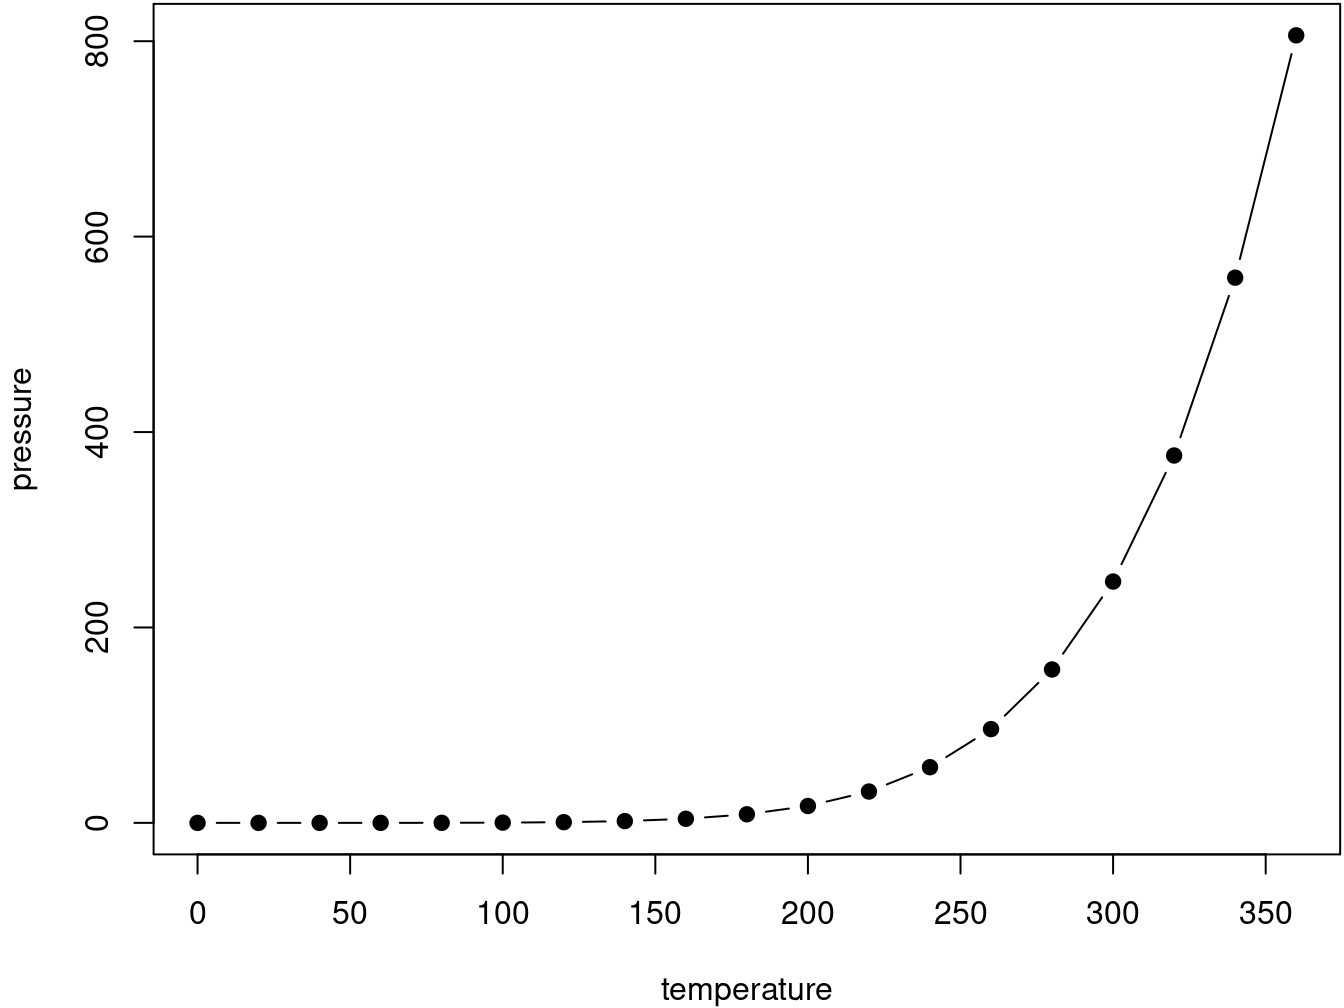
\includegraphics[width=0.8\linewidth]{data-science-practices-1_files/figure-latex/nice-fig-1} 

}

\caption{Here is a nice figure!}\label{fig:nice-fig}
\end{figure}

Reference a figure by its code chunk label with the \texttt{fig:} prefix, e.g., see Figure \ref{fig:nice-fig}. Similarly, you can reference tables generated from \texttt{knitr::kable()}, e.g., see Table \ref{tab:nice-tab}.

\begin{Shaded}
\begin{Highlighting}[]
\NormalTok{knitr}\OperatorTok{::}\KeywordTok{kable}\NormalTok{(}
  \KeywordTok{head}\NormalTok{(iris, }\DecValTok{20}\NormalTok{), }\DataTypeTok{caption =} \StringTok{'Here is a nice table!'}\NormalTok{,}
  \DataTypeTok{booktabs =} \OtherTok{TRUE}
\NormalTok{)}
\end{Highlighting}
\end{Shaded}

\begin{table}[t]

\caption{\label{tab:nice-tab}Here is a nice table!}
\centering
\begin{tabular}{rrrrl}
\toprule
Sepal.Length & Sepal.Width & Petal.Length & Petal.Width & Species\\
\midrule
5.1 & 3.5 & 1.4 & 0.2 & setosa\\
4.9 & 3.0 & 1.4 & 0.2 & setosa\\
4.7 & 3.2 & 1.3 & 0.2 & setosa\\
4.6 & 3.1 & 1.5 & 0.2 & setosa\\
5.0 & 3.6 & 1.4 & 0.2 & setosa\\
\addlinespace
5.4 & 3.9 & 1.7 & 0.4 & setosa\\
4.6 & 3.4 & 1.4 & 0.3 & setosa\\
5.0 & 3.4 & 1.5 & 0.2 & setosa\\
4.4 & 2.9 & 1.4 & 0.2 & setosa\\
4.9 & 3.1 & 1.5 & 0.1 & setosa\\
\addlinespace
5.4 & 3.7 & 1.5 & 0.2 & setosa\\
4.8 & 3.4 & 1.6 & 0.2 & setosa\\
4.8 & 3.0 & 1.4 & 0.1 & setosa\\
4.3 & 3.0 & 1.1 & 0.1 & setosa\\
5.8 & 4.0 & 1.2 & 0.2 & setosa\\
\addlinespace
5.7 & 4.4 & 1.5 & 0.4 & setosa\\
5.4 & 3.9 & 1.3 & 0.4 & setosa\\
5.1 & 3.5 & 1.4 & 0.3 & setosa\\
5.7 & 3.8 & 1.7 & 0.3 & setosa\\
5.1 & 3.8 & 1.5 & 0.3 & setosa\\
\bottomrule
\end{tabular}
\end{table}

You can write citations, too. For example, we are using the \textbf{bookdown} package \citep{R-bookdown} in this sample book, which was built on top of R Markdown and \textbf{knitr} \citep{xie2015}.

\bibliography{book.bib,packages.bib}


\end{document}
